% 无封面页
\documentclass[withoutpreface]{cumcmthesis}

\begin{document}

    %% 摘要页
    \begin{abstractpage}{基于层次分析法的旅游景点评价系统}
        
        本文主要解决如何确定评价指标、形成评价体系,为小明同学的旅游目的地进行合理的决策。

        针对所要研究的问题,我们选择了\textbf{层次分析法}进行建模。首先,我们通过网络途径确定了\textbf{景色}、\textbf{花费}、\textbf{居住}、\textbf{饮食}、\textbf{交通}这5个评价指标,并建立了包含目标层、准则层、方案层的层次结构模型。其次,经过主观猜测和网络数据对比,我们在因素间进行两两比较,构造了方案层关于准则层以及准则层关于目标层的\textbf{判断矩阵},并进行了\textbf{一致性检验}。6个判断矩阵均通过一致性检验。最后,我们基于判断矩阵分别以\textbf{算术平均法}、\textbf{几何平均法}、\textbf{特征值法}计算权重并进行了简单的算术平均。最终得到的旅游景点打分为:苏杭0.2992、北戴河0.2453、桂林0.4555。

        在层次分析法结果的基础之上,我们确定\textbf{桂林}即为最适合小明的旅游景点。
        \keywords{评价 \quad 权重 \quad 层次分析法 \quad 判断矩阵 \quad 一致性检验}

    \end{abstractpage}

    %% 目录页
    \tocpage

    \section{问题重述}

    填好志愿后, 小明同学决定出去旅游, 在查阅了网上的相关资料后,他初步选择了苏杭、北戴河和桂林作为目标景点的备选方案。

    我们的目的是\textbf{确定评价指标}、\textbf{形成评价体系},为小明同学选择最合适的方案。

    \section{问题分析}

    解决评价类问题,首先需要解决以下三个问题:
    \begin{enumerate}
        \item 评价问题的目标是什么?
        \item 为了达到评价目标,有哪几种待评价的方案?
        \item 评价进行的准则或指标是什么?
    \end{enumerate}

    一般而言,前两个问题的答案是显而易见的,而第三个问题的答案则需要我们结合\textbf{题目中的背景材料}、\textbf{常识}以及\textbf{网络上搜集到的参考资料},综合筛选后得出最适合的几个指标。

    具体而言,本文的评价目标是\textbf{选择最适合小明的旅游景点},待评价方案有\textbf{苏杭}、\textbf{北戴河}以及\textbf{桂林},评价指标则需要我们查找资料后\textbf{自行确定}。

    确定评价指标后,为了比较各个方案的优劣,作出合理的抉择,我们需要得出各个方案的优劣权重和各个指标的重要性权重。本文使用\textbf{层次分析法}。

    \section{模型假设}

    为了便于之后的建模分析,我们作出以下假设:

    \begin{itemize}
        \item 网络上搜集到的资料真实有效
    \end{itemize}

    \section{符号假设}

    在此对本文使用到的一些符号作以下说明(未作说明则在文中详述):

    \begin{table}[H]
        \centering
        \caption{符号假设}\label{Tab:12}
        \begin{tabular}{p{30pt}<{\centering}|p{100pt}<{\centering}@{}p{260pt}<{\centering}}
        \hline
        \rowcolor{color2} 序号 & 符号 & 符号说明 \\
        \hline
        \rowcolor{color1} 1 & $\mathbf{O}$		& 指标层对目标层的判断矩阵 \\
        \rowcolor{color1} 2 & $\mathbf{C_1,C_2,C_3,C_4,C_5}$		& 方案层对指标层的判断矩阵 \\
        \rowcolor{color1} 3 & $CI,RI,CR$		& 一致性检验相关指标\\
        \rowcolor{color1} 4 & $\omega$		& 权重向量 \\
        \hline
        \end{tabular}
    \end{table}

    \section{模型简介}

    层次分析法(The Analytic Hierarchy Process, 即 AHP)是由美国运筹学家、匹兹堡大学教授 T.L. Saaty 于20世纪70年代创立的一种系统分析与决策的综合评价方法,是在充分研究了人类思维过程的基础上提出来的,它较合理地解决了定性问题定量化的处理过程。

    AHP 的主要特点是通过建立递阶层次结构,把人类的判断转化到若因素两两之间重要度的比较上,从而把难于量化的定性判断转化为可操作的重要度的比较上面。在许多情况下,决策者可以直接使用AHP进行决策,极大地提高了决策的有效性、可靠性和可行性,但其本质是一种思维方式,它把复杂问题分解成多个组成因素,又将这些因素按支配关系分别形成递阶层次结构,通过两两比较的方法确定决策方案相对重要度的总排序。整个过程体现了人类决策思维的基本特征,即分解、判断、综合,克服了其他方法回避决策者主观判断的缺点。

    \section{模型建立}

    \subsection{建立层次结构模型}

    查找资料后,我们确定了五个评价指标:\textbf{景色}、\textbf{花费}、\textbf{居住}、\textbf{饮食}、\textbf{交通}。于是,评价问题转化为填写\cref{Tab:1}:计算5个指标相关于“最佳旅游景点”的重要性权重,计算3个旅游景点相关于5个指标的优秀权重。

    \begin{table}[H]
        \centering
        \caption{评价问题需要填写的表格}\label{Tab:1}
        \begin{tabular}{|p{1.5cm}<{\centering}|p{2cm}<{\centering}|p{1.5cm}<{\centering}|p{1.5cm}<{\centering}|p{1.5cm}<{\centering}|}
        \hline
        &  指标权重 & 苏杭 & 北戴河 & 桂林 \\
        \hline
        景色   & \cellcolor{color9} & \cellcolor{color6} & \cellcolor{color6} & \cellcolor{color6} \bigstrut\\
        \hline
        花费   & \cellcolor{color9} & \cellcolor{color10} & \cellcolor{color10} & \cellcolor{color10} \bigstrut\\
        \hline
        居住   & \cellcolor{color9} & \cellcolor{color4} & \cellcolor{color4} & \cellcolor{color4} \bigstrut\\
        \hline
        饮食& \cellcolor{color9} & \cellcolor{color12} & \cellcolor{color12} & \cellcolor{color12} \\
        \hline
        交通& \cellcolor{color9} & \cellcolor{color8} & \cellcolor{color8} & \cellcolor{color8} \\
        \hline
        \end{tabular}
    \end{table}

    进一步,在分析了各指标之间的关系的基础上,我们建立了如\cref{Fig:1}的递阶层次结构模型。其中,准则层由5个独立指标组成,方案层则包含3个方案。评价问题转化为分别计算方案层关于准则层,准则层关于目标层的权重,最后根据这些权重计算方案层关于目标层的权重。

    \begin{figure}[H]
        \centering
        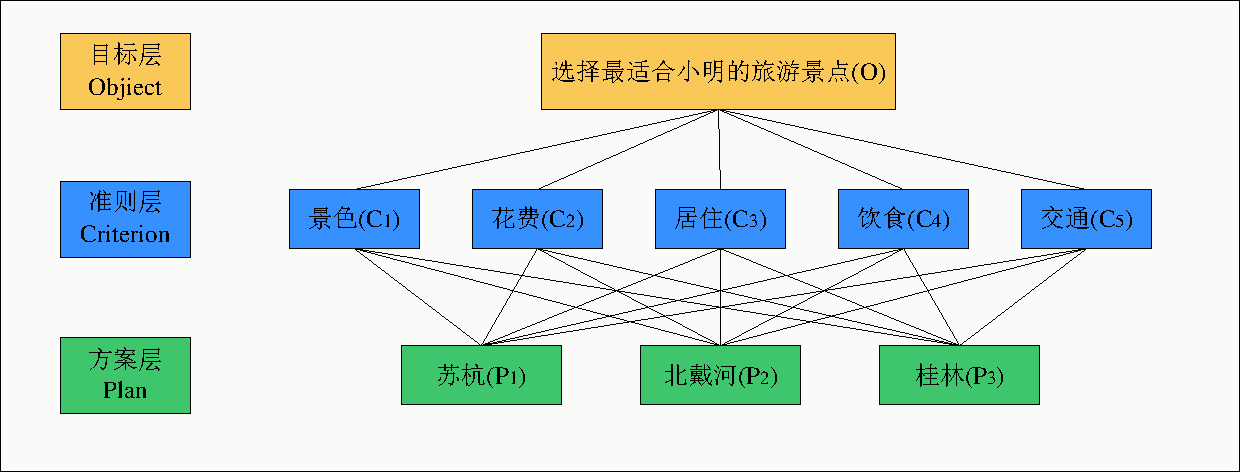
\includegraphics[width=\textwidth]{层次分析图}
        \caption{递阶层次结构模型图}\label{Fig:1}
    \end{figure}

    \subsection{构建判断矩阵}

    \begin{table}[H]
        \centering
        \caption{重要性程度度量表}\label{Tab:3}
        \begin{tabular}{cc}
            \toprule[1.5pt]
            \makebox[0.2\textwidth][c]{标度} & \makebox[0.6\textwidth][c]{含义} \\
            \midrule
            1 &  两个因素相比,具有相同的重要性\\
            3 &  两个因素相比,一个因素比另一个因素稍微重要\\
            5 & 两个因素相比,一个因素比另一个因素明显重要\\
            7 & 两个因素相比,一个因素比另一个因素强烈重要 \\
            9 & 两个因素相比,一个因素比另一个因素极端重要 \\
            2、4、6、8 &  以上指标的中值\\
            倒数 & 因素A与因素B为a,则因素B与因素A为$\frac{1}{a}$\\ 
            \bottomrule[1.5pt]
        \end{tabular}
    \end{table}

    首先整理查找得到的资料,按照重要性程度度量\cref{Tab:3},对方案层的3个旅游景点进行关于准则层5个指标的两两比较,构建方案层关于准则层各指标的两两判断矩阵,共有5个,即$\mathbf{C_1},\mathbf{C_2},\mathbf{C_3},\mathbf{C_4},\mathbf{C_5},$。如\cref{Tab:2}所示。

    \begin{table}[H]
        \centering
        \caption{方案层关于准则层各指标的判断矩阵}\label{Tab:2}
        \begin{tabular}{|p{0.7cm}<{\centering}|p{0.7cm}<{\centering}|p{0.7cm}<{\centering}|p{0.7cm}<{\centering}|}
            \hline
            $\color{color11} \mathbf{C_1}$ & $P_1$ & $P_2$ & $P_3$ \\ 
            \hline
            $P_1$ & \cellcolor{color5} 1 & \cellcolor{color4} 2 & \cellcolor{color4} 5 \\
            \hline
            $P_2$ & \cellcolor{color1} $\frac{1}{2}$ & \cellcolor{color5} 1 & \cellcolor{color4} 2\\
            \hline
            $P_3$ & \cellcolor{color1} $\frac{1}{5}$ & \cellcolor{color1} $\frac{1}{2}$ & \cellcolor{color5} 1\\
            \hline 
        \end{tabular}
        \begin{tabular}{|p{0.7cm}<{\centering}|p{0.7cm}<{\centering}|p{0.7cm}<{\centering}|p{0.7cm}<{\centering}|}
            \hline
            $\color{color11} \mathbf{C_2}$ & $P_1$ & $P_2$ & $P_3$ \\ 
            \hline
            $P_1$ & \cellcolor{color5} 1 & \cellcolor{color4} $\frac{1}{3}$ & \cellcolor{color4} $\frac{1}{8}$ \\
            \hline
            $P_2$ & \cellcolor{color1} 3 & \cellcolor{color5} 1 & \cellcolor{color4} $\frac{1}{3}$\\
            \hline
            $P_3$ & \cellcolor{color1} 8 & \cellcolor{color1} 3 & \cellcolor{color5} 1\\
            \hline 
        \end{tabular}
        \begin{tabular}{|p{0.7cm}<{\centering}|p{0.7cm}<{\centering}|p{0.7cm}<{\centering}|p{0.7cm}<{\centering}|}
            \hline
            $\color{color11} \mathbf{C_3}$ & $P_1$ & $P_2$ & $P_3$ \\ 
            \hline
            $P_1$ & \cellcolor{color5} 1 & \cellcolor{color4} 1 & \cellcolor{color4} 3 \\
            \hline
            $P_2$ & \cellcolor{color1} 1 & \cellcolor{color5} 1 & \cellcolor{color4} 3\\
            \hline
            $P_3$ & \cellcolor{color1} $\frac{1}{3}$ & \cellcolor{color1} $\frac{1}{3}$ & \cellcolor{color5} 1\\
            \hline 
        \end{tabular}

        \vspace{4pt}
        \begin{tabular}{|p{0.7cm}<{\centering}|p{0.7cm}<{\centering}|p{0.7cm}<{\centering}|p{0.7cm}<{\centering}|}
            \hline
            $\color{color11} \mathbf{C_4}$ & $P_1$ & $P_2$ & $P_3$ \\ 
            \hline
            $P_1$ & \cellcolor{color5} 1 & \cellcolor{color4} 3 & \cellcolor{color4} 4 \\
            \hline
            $P_2$ & \cellcolor{color1} $\frac{1}{3}$ & \cellcolor{color5} 1 & \cellcolor{color4} 1\\
            \hline
            $P_3$ & \cellcolor{color1} $\frac{1}{4}$ & \cellcolor{color1} 1 & \cellcolor{color5} 1\\
            \hline 
        \end{tabular}
        \begin{tabular}{|p{0.7cm}<{\centering}|p{0.7cm}<{\centering}|p{0.7cm}<{\centering}|p{0.7cm}<{\centering}|}
            \hline
            $\color{color11} \mathbf{C_5}$ & $P_1$ & $P_2$ & $P_3$ \\ 
            \hline
            $P_1$ & \cellcolor{color5} 1 & \cellcolor{color4} 1 & \cellcolor{color4} $\frac{1}{4}$ \\
            \hline
            $P_2$ & \cellcolor{color1} 1 & \cellcolor{color5} 1 & \cellcolor{color4} $\frac{1}{4}$ \\
            \hline
            $P_3$ & \cellcolor{color1} 4 & \cellcolor{color1} 4 & \cellcolor{color5} 1\\
            \hline 
        \end{tabular}
    \end{table}

    其次,根据主观猜测,构建准则层5个指标关于目标层的两两判断矩阵$\mathbf{O}$。如\cref{Tab:4}所示。

    \begin{table}[H]
        \centering
        \caption{准则层关于目标层的两两判断矩阵}\label{Tab:4}
        \begin{tabular}{|p{0.7cm}<{\centering}|p{0.7cm}<{\centering}|p{0.7cm}<{\centering}|p{0.7cm}<{\centering}|p{0.7cm}<{\centering}|p{0.7cm}<{\centering}|}
            \hline
            $\color{color11} \mathbf{O}$ & $C_1$ & $C_2$ & $C_3$ & $C_4$ & $C_5$ \\ 
            \hline
            $C_1$ & \cellcolor{color5} 1 & \cellcolor{color12} $\frac{1}{2}$ & \cellcolor{color12} 4 &\cellcolor{color12} 3 & \cellcolor{color12} 3\\
            \hline
            $C_2$ & \cellcolor{color1} 2 & \cellcolor{color5} 1 & \cellcolor{color12} 7 & \cellcolor{color12} 5 & \cellcolor{color12} 5 \\
            \hline
            $C_3$ & \cellcolor{color1} $\frac{1}{4}$ & \cellcolor{color1} $\frac{1}{7}$ & \cellcolor{color5} 1 & \cellcolor{color12} $\frac{1}{2}$ & \cellcolor{color12} $\frac{1}{3}$\\
            \hline 
            $C_4$ & \cellcolor{color1} $\frac{1}{3}$ & \cellcolor{color1} $\frac{1}{5}$ & \cellcolor{color1} 2 & \cellcolor{color5} 1 & \cellcolor{color12} 1\\
            \hline 
            $C_5$ & \cellcolor{color1} $\frac{1}{3}$ & \cellcolor{color1} $\frac{1}{5}$ & \cellcolor{color1} 3 & \cellcolor{color1} 1 & \cellcolor{color5} 1\\
            \hline 
        \end{tabular}
    \end{table}

    \subsection{一致性检验}

    为了检验我们构造的判断矩阵是否接近于一致矩阵,我们需要进行一致性检验。

    首先,计算\textbf{一致性指标}$CI$。$CI$的计算公式如下:
    \begin{equation}
        CI = \frac{\lambda_{max}-n}{n-1}
    \end{equation}

    其中,$\lambda_{max}$是方阵的最大特征值,$n$是方阵的维数。

    \begin{table}[H]
        \centering
        \caption{$CI$计算结果}\label{Tab:5}
        \begin{tabular}{*{6}{p{2cm}<\centering}}
            \toprule[1.1pt] 
            $\mathbf{C_1}$ & $\mathbf{C_2}$ & $\mathbf{C_3}$ & $\mathbf{C_4}$ & $\mathbf{C_5}$ & $\mathbf{O}$\\
            \midrule
            0.0027676 & 0.00077081 & 0 & 0.0046014 & 0 & 0.018021\\  
            \bottomrule[1.1pt]
        \end{tabular}
    \end{table}

    其次,查询\textbf{平均随机一致性指标}表得$n=3$时,平均随机一致性指标$RI=0.52$;$n=5$时,平均随机一致性指标$RI=1.12$。

    \begin{table}[H]
        \centering
        \caption{$RI$查询表}\label{Tab:6}
        \begin{tabular}{*{13}{p{0.73cm}<\centering}}
            \toprule[1.1pt] 
            $\mathbf{n}$ & \cellcolor{color11} 3 & 4 & \cellcolor{color11} 5 & 6 & 7 & 8 & 9 & 10 & 11 & 12 & 13 & 14 \\ 
            \midrule
            $\mathbf{RI}$ & \cellcolor{color11} 0.52 & 0.89 & \cellcolor{color11} 1.12 & 1.26 & 1.36 & 1.41 & 1.46 & 1.49 & 1.52 & 1.54 & 1.56 & 1.58 \\ 
            \bottomrule[1.1pt]
        \end{tabular}
    \end{table}

    最后,计算{一致性比例}$CR$:
    \begin{equation}
        CR = \frac{CI}{RI}
    \end{equation}

    \begin{table}[H]
        \centering
        \caption{$CR$计算结果}\label{Tab:7}
        \begin{tabular}{*{6}{p{2cm}<\centering}}
            \toprule[1.1pt] 
            $\mathbf{C_1}$ & $\mathbf{C_2}$ & $\mathbf{C_3}$ & $\mathbf{C_4}$ & $\mathbf{C_5}$ & $\mathbf{O}$\\
            \midrule
            0.0053222 & 0.0014823 & 0 & 0.0088488 & 0 & 0.01609\\  
            \bottomrule[1.1pt]
        \end{tabular}
    \end{table}

    $CR<0.1$,说明判断矩阵的一致性可以接受;否则则需要重新构造判断矩阵。我们的6个判断矩阵均通过一致性检验,可以进行后续的权重计算。

    \subsection{权重计算}

    判断矩阵已经通过了一致性检验,说明我们可以基于这些判断矩阵进行权重计算。权重计算主要有3种方法:算术平均法、几何平均法、特征值法。

    \subsubsection{算术平均法}

    算术平均法求权重的步骤如下:

    \begin{enumerate}
        \item 将判断矩阵按列进行归一化
        \item 将归一化的各列相加
        \item 将相加后的结果向量除以方阵的维数$n$
    \end{enumerate}

    假设判断矩阵为$$A=\begin{bmatrix}
        a_{11} & a_{12} & \cdots & a_{1n} \\
        a_{21} & a_{2} & \cdots & a_{2n} \\
        \vdots & \vdots & \ddots & \vdots \\
        a_{n1} & a_{n2} & \cdots & a_{nn} \\ 
    \end{bmatrix}$$
    那么算术平均法求得的权重为
    \begin{equation}
        \omega_i = \frac{1}{n} \sum\limits_{j=1}^{n} \frac{a_{ij}}{\sum\limits_{k=1}^{n}a_{kj}}
    \end{equation}

    \subsubsection{几何平均法}

    几何平均法求权重的步骤如下:
    \begin{enumerate}
        \item 将判断矩阵各列相乘得到一个列向量
        \item 将结果向量的每个分量开 n 次根
        \item 对结果向量进行归一化
    \end{enumerate}

    假设判断矩阵为$$A=\begin{bmatrix}
        a_{11} & a_{12} & \cdots & a_{1n} \\
        a_{21} & a_{2} & \cdots & a_{2n} \\
        \vdots & \vdots & \ddots & \vdots \\
        a_{n1} & a_{n2} & \cdots & a_{nn} \\ 
    \end{bmatrix}$$
    那么算术平均法求得的权重为
    \begin{equation}
        \omega_i = \frac{(\prod \limits_{j=1}^n a_{ij})^{\frac{1}{n}}}{\sum\limits_{k=1}^{n} (\prod \limits_{j=1}^n a_{kj})^{\frac{1}{n}}}
    \end{equation}

    \subsubsection{特征值法}

    特征值法求权重的步骤如下:

    \begin{enumerate}
        \item 求出判断矩阵的特征值及特征向量
        \item 从中挑选最大特征值并将对应的特征向量进行归一化
    \end{enumerate}

    \subsubsection{结果平均汇总}

    为了保持模型的稳健性,我们将三种方法得到的权重进行汇总,并进行简单的算术平均。

    
    \begin{table}[H]
        \centering
        \caption{目标层权重计算结果}\label{Tab:8}
        \begin{tabular}{|c|c|c|c|c|}
            \hline
            $\color{color11} \mathbf{C_1}$& 算术平均法 & 几何平均法 & 特征值法 & 平均值 \\
            \hline
            景色 & 0.5949 & 0.5954 & 0.5954 & 0.5952 \\ 
            \hline
            花费 & 0.2766 & 0.2764  & 0.2764 & 0.2764  \\ 
            \hline
            居住 & 0.1285 & 0.1283 & 0.1283 & 0.1283  \\ 
            \hline
        \end{tabular}

        \vspace{3pt}
        \begin{tabular}{|c|c|c|c|c|}
            \hline
            $\color{color11} \mathbf{C_2}$& 算术平均法 & 几何平均法 & 特征值法 & 平均值 \\
            \hline
            景色 & 0.0820  & 0.0819 & 0.0819 & 0.0820 \\ 
            \hline
            花费 & 0.2364 & 0.2363 & 0.2363 & 0.2364 \\ 
            \hline
            居住 & 0.6816 & 0.6817 & 0.6817 & 0.6817 \\ 
            \hline
        \end{tabular}

        \vspace{3pt}
        \begin{tabular}{|c|c|c|c|c|}
            \hline
            $\color{color11} \mathbf{C_3}$& 算术平均法 & 几何平均法 & 特征值法 & 平均值 \\
            \hline
            景色 & 0.4286 & 0.4286 & 0.4286 & 0.4286 \\ 
            \hline
            花费 & 0.4286 & 0.4286 & 0.4286 & 0.4286 \\ 
            \hline
            居住 & 0.1429 & 0.1429 & 0.1429 & 0.1429 \\ 
            \hline
        \end{tabular}

        \vspace{3pt}
        \begin{tabular}{|c|c|c|c|c|}
            \hline
            $\color{color11} \mathbf{C_4}$& 算术平均法 & 几何平均法 & 特征值法 & 平均值 \\
            \hline
            景色 &  0.6327 & 0.6337 & 0.6337 & 0.6334 \\ 
            \hline
            花费 & 0.1924  & 0.1919 & 0.1919 & 0.1921 \\ 
            \hline
            居住 & 0.1749 & 0.1744 & 0.1744 & 0.1745 \\ 
            \hline
        \end{tabular}

        \vspace{3pt}
        \begin{tabular}{|c|c|c|c|c|}
            \hline
            $\color{color11} \mathbf{C_5}$& 算术平均法 & 几何平均法 & 特征值法 & 平均值 \\
            \hline
            景色 & 0.1667 & 0.1667 & 0.1667 & 0.1667 \\ 
            \hline
            花费 & 0.1667 & 0.1667 & 0.1667  & 0.1667 \\ 
            \hline
            居住 & 0.6667 & 0.6667 & 0.6667 & 0.6667 \\ 
            \hline
        \end{tabular}
    \end{table}

    \begin{table}[H]
        \centering
        \caption{准则层权重计算结果}\label{Tab:9}
        \begin{tabular}{|p{1cm}<{\centering}*{4}{|p{2.5cm}<{\centering}}|}
            \hline
            $\color{color11} \mathbf{O}$ & 算术平均法 & 几何平均法 & 特征值法 & 平均值 \\
            \hline
            景色 & 0.2623 & 0.2636 & 0.2636 & 0.2632\\ 
            \hline
            花费 & 0.4744 & 0.4773 & 0.4758 & 0.4758\\ 
            \hline
            居住 & 0.0545 & 0.0531 & 0.0538  & 0.0538\\ 
            \hline
            饮食 & 0.0985 & 0.0988 & 0.0981 & 0.0985 \\ 
            \hline
            交通 & 0.1103 & 0.1072 & 0.1087 & 0.1087 \\ 
            \hline
        \end{tabular}
    \end{table}

    综上,我们实际上已经填完了\cref{Tab:1}。经过最后一步加权计算,我们得到了最终的旅游景点打分结果。经过对比,我们可以作出决策:权重最高(=0.4555)的\textbf{桂林}是最适合小明的旅游景点。

    \begin{table}[H]
        \centering
        \caption{权重汇总表}\label{Tab:10}
        \begin{tabular}{|p{1.5cm}<{\centering}|p{2cm}<{\centering}|p{1.5cm}<{\centering}|p{1.5cm}<{\centering}|p{1.5cm}<{\centering}|}
        \hline
        &  指标权重 & 苏杭 & 北戴河 & 桂林 \\
        \hline
        景色   & \cellcolor{color9} 0.2632 & \cellcolor{color6} 0.5952 & \cellcolor{color6} 0.2764 & \cellcolor{color6}  0.1283 \bigstrut\\
        \hline
        花费   & \cellcolor{color9} 0.4758 & \cellcolor{color4} 0.0820 & \cellcolor{color4} 0.2364 & \cellcolor{color4}  0.6817 \bigstrut\\
        \hline
        居住   & \cellcolor{color9} 0.0538 & \cellcolor{color10} 0.4286 & \cellcolor{color10} 0.4286 & \cellcolor{color10} 0.1429 \bigstrut\\
        \hline
        饮食& \cellcolor{color9} 0.0985 & \cellcolor{color12} 0.6334 & \cellcolor{color12}  0.1921 & \cellcolor{color12}  0.1745 \\
        \hline
        交通& \cellcolor{color9} 0.1087 & \cellcolor{color8} 0.1667 & \cellcolor{color8} 0.1667 & \cellcolor{color8} 0.6667 \\
        \hline
        \end{tabular}
    \end{table}

    \begin{table}[H]
        \centering
        \caption{各旅游景点最终打分}\label{Tab:11}
        \begin{tabular}{*{3}{p{1.5cm}<\centering}}
            \toprule[1.1pt] 
            苏杭 & 北戴河 & 桂林 \\ 
            \midrule
            0.2992 & 0.2453 & 0.4555 \\  
            \bottomrule[1.1pt]
        \end{tabular}
    \end{table}
    

    \section{模型评价}
    \subsection{优点}
    \begin{enumerate}
        \item 层次分析法可以处理定量和定性结合的问题
        \item 层次分析法简洁实用
        \item 层次分析法所需定量数据少
    \end{enumerate}


    \subsection{局限}
    \begin{enumerate}
        \item 层次分析法只能在指定方案中进行选择,无法发掘新的方案
        \item 评价体系过于主观,需要专家系统的支持,如果指标不合理,最后得到的结果也会不准确
        \item 方案层不能过多,否则能够通过一致性检验的判断矩阵难以构造
    \end{enumerate}

    \appendix

    \section{Matlab代码}
    \begin{lstlisting}[language=matlab,caption={AHPConsistencyCheck.m}]
    function [pass,weights,CI,RI,CR] = AHPConsistencyCheck(A)
    % 层次分析法(AHP)中对判断矩阵A进行一致性检验并计算权重
    % [pass,weights,CI,RI,CR] = AHPConsistencyCheck(A)
    % pass=true表示通过一致性检验,pass=false则为未通过
    % weights:返回的权重矩阵。
    % 从左到右各列分别为算术平均法、几何平均法、特征值法、平均值
    % CI,RI,CR:相关检验量
    % A:判断矩阵
        
        %% 判断矩阵是否为方阵
        [m,n] = size(A); 
        if m ~= n
            disp("判断矩阵应为方阵,但输入为(" + num2str(m) + "," ...
                + num2str(n) + ")");
        end

        %% 一致性检验
        [X,Lambda]=eig(A);  % 求特征值和特征向量

        % 寻找最大特征值及对应的特征向量
        lambda = Lambda(1,1);
        indexOFlambda = 1;
        for i=2:n
            if Lambda(i,i) > lambda
                lambda = Lambda(i,i);
                indexOFlambda = i;
            end
        end
        x = X(:,indexOFlambda);
        
        % 计算CI,查询RI,计算CR
        CI = (lambda - n)/(n - 1);
        RItable = [0,0,0.52,0.89,1.12,1.26,1.36,1.41,1.46,...
            1.49,1.52,1.54,1.56,1.58];
        RI=RItable(n);
        CR = CI/RI;
        
        % 判断是否通过一致性检验
        if CR >= 0.1
            pass = false;
            weights = [];
            return 
        else
            pass = true;
        end

        %% 算术平均法
        % 各列归一化
        for i=1:n
            A(:,i) = A(:,i) / sum(A(:,i));
        end
        % 各列求算术平均
        origin_weight = sum(A,2);
        weights = origin_weight / sum(origin_weight);

        %% 几何平均法
        % 各列求几何平均
        origin_weight = A(:,1);
        for i=2:n
            origin_weight = origin_weight .* A(:,i);
        end
        origin_weight = origin_weight.^(1/n);
        % 结果向量归一化
        weights = [ weights , origin_weight / sum(origin_weight)];
        
        %% 特征值法
        origin_weight = x;
        weights = [ weights , origin_weight / sum(origin_weight)];
        
        %% 平均值
        weights = [ weights , sum(weights,2) / 3];
    end
    \end{lstlisting}

    \begin{lstlisting}[language=matlab,caption={drawWeights.m}]
    function  drawWeights(weights,labels)
    % 绘制权重图
    % weights:权重行向量或列向量
    % labels:数据标签

        n = length(weights);
        weights = weights / sum(weights);
        facecolor = "#3691ff";
        width = 0.3;
        barh(weights,FaceColor=facecolor,BarWidth=width);
        xlim([0,3/2*max(weights)]);
        yticks(1:n)
        yticklabels(labels);
        for i=1:n
            text(weights(i)+1/100*max(weights),i,num2str(weights(i)))
        end

    end
    \end{lstlisting}
    
    \begin{lstlisting}[language=matlab,caption={main.m}]
    % 通过层次分析法选择最佳旅游地

    clear,clc
    
    %% 输入判断矩阵
    
    % 准则层对目标层
    O = [1 1/2 4 3 3
        2 1 7 5 5
        1/4 1/7 1 1/2 1/3
        1/3 1/5 2 1 1
        1/3 1/5 3 1 1];
    
    % 方案层对准则层
    C1 = [1 2 5; 1/2 1 2; 1/5 1/2 1];
    C2 = [1 1/3 1/8; 3 1 1/3; 8 3 1];
    C3 = [1 1 3; 1 1 3; 1/3 1/3 1];
    C4 = [1 3 4; 1/3 1 1; 1/4 1 1];
    C5 = [1 1 1/4; 1 1 1/4; 4 4 1];
    
    Mats = {O,C1,C2,C3,C4,C5};
    MatNum = size(Mats,2);
    Weights = cell(1,MatNum);
    
    %% 一致性检验及权重计算
    for i=1:MatNum
        [pass,weights,CI,RI,CR] = AHPConsistencyCheck(Mats{i});
        Weights{i} = weights;
        if pass
            disp("第" + num2str(i) + "个矩阵通过一致性检验");
            disp("CI=" + num2str(CI) + "  RI=" + num2str(RI) ...
                + "  CR=" + num2str(CR) + "<0.1");
            disp("权重表为:");
            disp(weights);
        else
            disp("第" + num2str(i) + "个矩阵未通过一致性检验");
            disp("CI=" + num2str(CI) + "  RI=" + num2str(RI) ...
                + "CR=" + num2str(CR) + ">=0.1");
        end
    end
    
    %% 权重汇总表
    weightsTable = ones(5,4);
    weightsTable(:,1) = Weights{1,1}(:,end);
    for i=2:MatNum
        weightsTable(i-1,2:end) = Weights{1,i}(:,end);
    end
    disp("权重汇总表:");
    disp(weightsTable);
    
    %% 计算最终打分
    grades = ones(3,1);
    for i=1:3
        grades(i,1) = weightsTable(:,1)' * weightsTable(:,i+1);
    end
    disp("最终得分:");
    disp(grades);
    
    %% 可视化
    [sortedGrades,sortedLabels] = sortWeights(grades,["苏杭","北戴河","桂林"]);
    drawWeights(sortedGrades,sortedLabels);
    
    clear O C1 C2 C3 C4 C5 pass CI RI CR weights i MatNum 
        

    \end{lstlisting}

    \section{Python 代码}

    \begin{lstlisting}[language=python,caption={初始化}]
    import numpy as np
    import matplotlib.pyplot as plt

    np.set_printoptions(precision=4)
    import matplotlib.pyplot as plt
    plt.rcParams["font.sans-serif"]=["SimHei"] #设置字体
    plt.rcParams["axes.unicode_minus"]=False # 解决图像中的“-”负号的乱码问题

    C1 = np.array([[1, 2, 5], [1 / 2, 1, 2], [1 / 5, 1 / 2, 1]])
    C2 = np.array([[1, 1 / 3, 1 / 8], [3, 1, 1 / 3], [8, 3, 1]])
    C3 = np.array([[1, 1, 3], [1, 1, 3], [1 / 3, 1 / 3, 1]])
    C4 = np.array([[1, 3, 4], [1 / 3, 1, 1], [1 / 4, 1, 1]])
    C5 = np.array([[1, 1, 1 / 4], [1, 1, 1 / 4], [4, 4, 1]])
    print(C1,C2,C3,C4,C5,sep="\n\n")

    O = np.array([[1, 1 / 2, 4, 3, 3], [2, 1, 7, 5, 5],
              [1 / 4, 1 / 7, 1, 1 / 2, 1 / 3], [1 / 3, 1 / 5, 2, 1, 1],
              [1 / 3, 1 / 5, 3, 1, 1]])
    print(O)
    \end{lstlisting}

    \begin{lstlisting}[language=python,caption={AHPConsistencyCheck函数}]
    def AHPConsistencyCheck(A):
    """对判断矩阵进行一致性检验并计算权重"""

        A = A.copy()
        ## 判断是否非方阵
        m, n = A.shape
        if m != n:
            print(f"判断矩阵应为方阵。但输入矩阵为({m},{n})")
            return False, None, None, None, None

        ## 一致性检验
        # 计算特征向量和特征值
        Lambdas, X = np.linalg.eig(A)
        LambdaIndex = np.argmax(Lambdas)
        Lambda, x = np.real(Lambdas[LambdaIndex]), np.real(X[:, LambdaIndex])

        # 计算CI,RI,CR
        CI = (Lambda - n) / (n - 1)
        RITable = [
            0, 0, 0.52, 0.89, 1.12, 1.26, 1.36, 1.41, 1.46, 1.49, 1.52, 1.54, 1.56,
            1.58
        ]
        RI = RITable[n - 1]
        CR = CI / RI

        # 判断是否通过一致性检验
        if CR >= 0.1:
            return False, None, CI, RI, CR
        else:
            Pass = True

        ## 算术平均法
        # 各列归一化
        for i in range(n):
            A[:, i] = A[:, i] / np.sum(A[:, i])
        # 各列求算术平均
        origin_weights = np.sum(A, 1).reshape((-1, 1))
        weights = origin_weights / sum(origin_weights)

        ## 几何平均法
        # 各列求几何平均
        origin_weights = np.prod(A, 1)
        origin_weights = origin_weights.reshape((-1, 1))
        origin_weights = origin_weights**(1 / n)
        weights = np.concatenate([weights, origin_weights / sum(origin_weights)],
                                1)

        ## 特征值法
        weights = np.concatenate([weights, x.reshape(-1, 1) / np.sum(x)], 1)

        ## 平均值
        weights = np.concatenate(
            [weights, np.sum(weights, 1).reshape(-1, 1) / 3], 1)
        return Pass, weights, CI, RI, CR
    \end{lstlisting}
    
    \begin{lstlisting}[language=python,caption={sortWeights函数}]
    def sortWeights(weights, labels):
    """从小到大排序权重和标签"""

        weights = weights / sum(weights)
        wl = list(zip(weights, labels))
        wl.sort(key=lambda x: x[0])
        sortedWeights, sortedLabels = zip(*wl)
        sortedWeights = np.array(sortedWeights)
        sortedLabels = list(sortedLabels)
        return sortedWeights, sortedLabels
    \end{lstlisting}

    \begin{lstlisting}[language=python,caption={drawWeights函数}]
    def drawWeights(weights, labels):
    """绘制权重图"""
        n = len(weights)
        ax=plt.axes()
        ax.set_facecolor("#FAFAF8")
        ax.barh([i for i in range(1,
                                   len(weights) + 1)],
                 weights,
                 height=0.2,
                 color="#3691ff")
        y = [i for i in range(1, n + 1)]
        plt.yticks(y, labels)
        plt.xlim(0, 1)
        for i in range(n):
            plt.text(weights[i] + 0.01, y[i] - 0.03, weights[i])
    \end{lstlisting}

    \begin{lstlisting}[language=python,caption={AHP主体}]
    Mats = [O, C1, C2, C3, C4, C5]

    # 一致性检验
    Weights = []
    for i in range(len(Mats)):
        Pass, weights, CI, RI, CR = AHPConsistencyCheck(Mats[i])
        Weights.append(weights)
        if Pass:
            print(f"第{i+1}个矩阵通过一致性检验")
            print(f"CI={CI:.6f}  RI={RI:.2f}  CR={CR:.6f}<0.1")
            print(f"权重表为:\n{weights}\n")
        else:
            print(f"第{i+1}个矩阵未通过一致性检验!!!")
            print(f"CI={CI:.6f}  RI={RI:.2f}  CR={CR:.6f}>=0.1\n")
    
    # 权重汇总表
    weightsTable = np.ones(shape=(5, 4))
    weightsTable[:, 0] = Weights[0][:, -1]
    for i in range(1, len(Mats)):
        weightsTable[i - 1, 1:] = Weights[i][:, -1]
    print(f"权重汇总表:\n{weightsTable}\n")

    # 最终打分计算
    grades = np.ones(3)

    for i in range(3):
        grades[i] = np.dot(weightsTable[:, 0].T, weightsTable[:, i + 1])
    print(f"最终得分:\n{grades}\n")

    # 可视化
    sortedWeights,sortedLabels = sortWeights(grades,["苏杭","北戴河","杭州"])
    drawWeights(np.round(sortedWeights,4),sortedLabels)        
    \end{lstlisting}


\end{document}